%!TEX ROOT=main.tex

\begin{figure}
    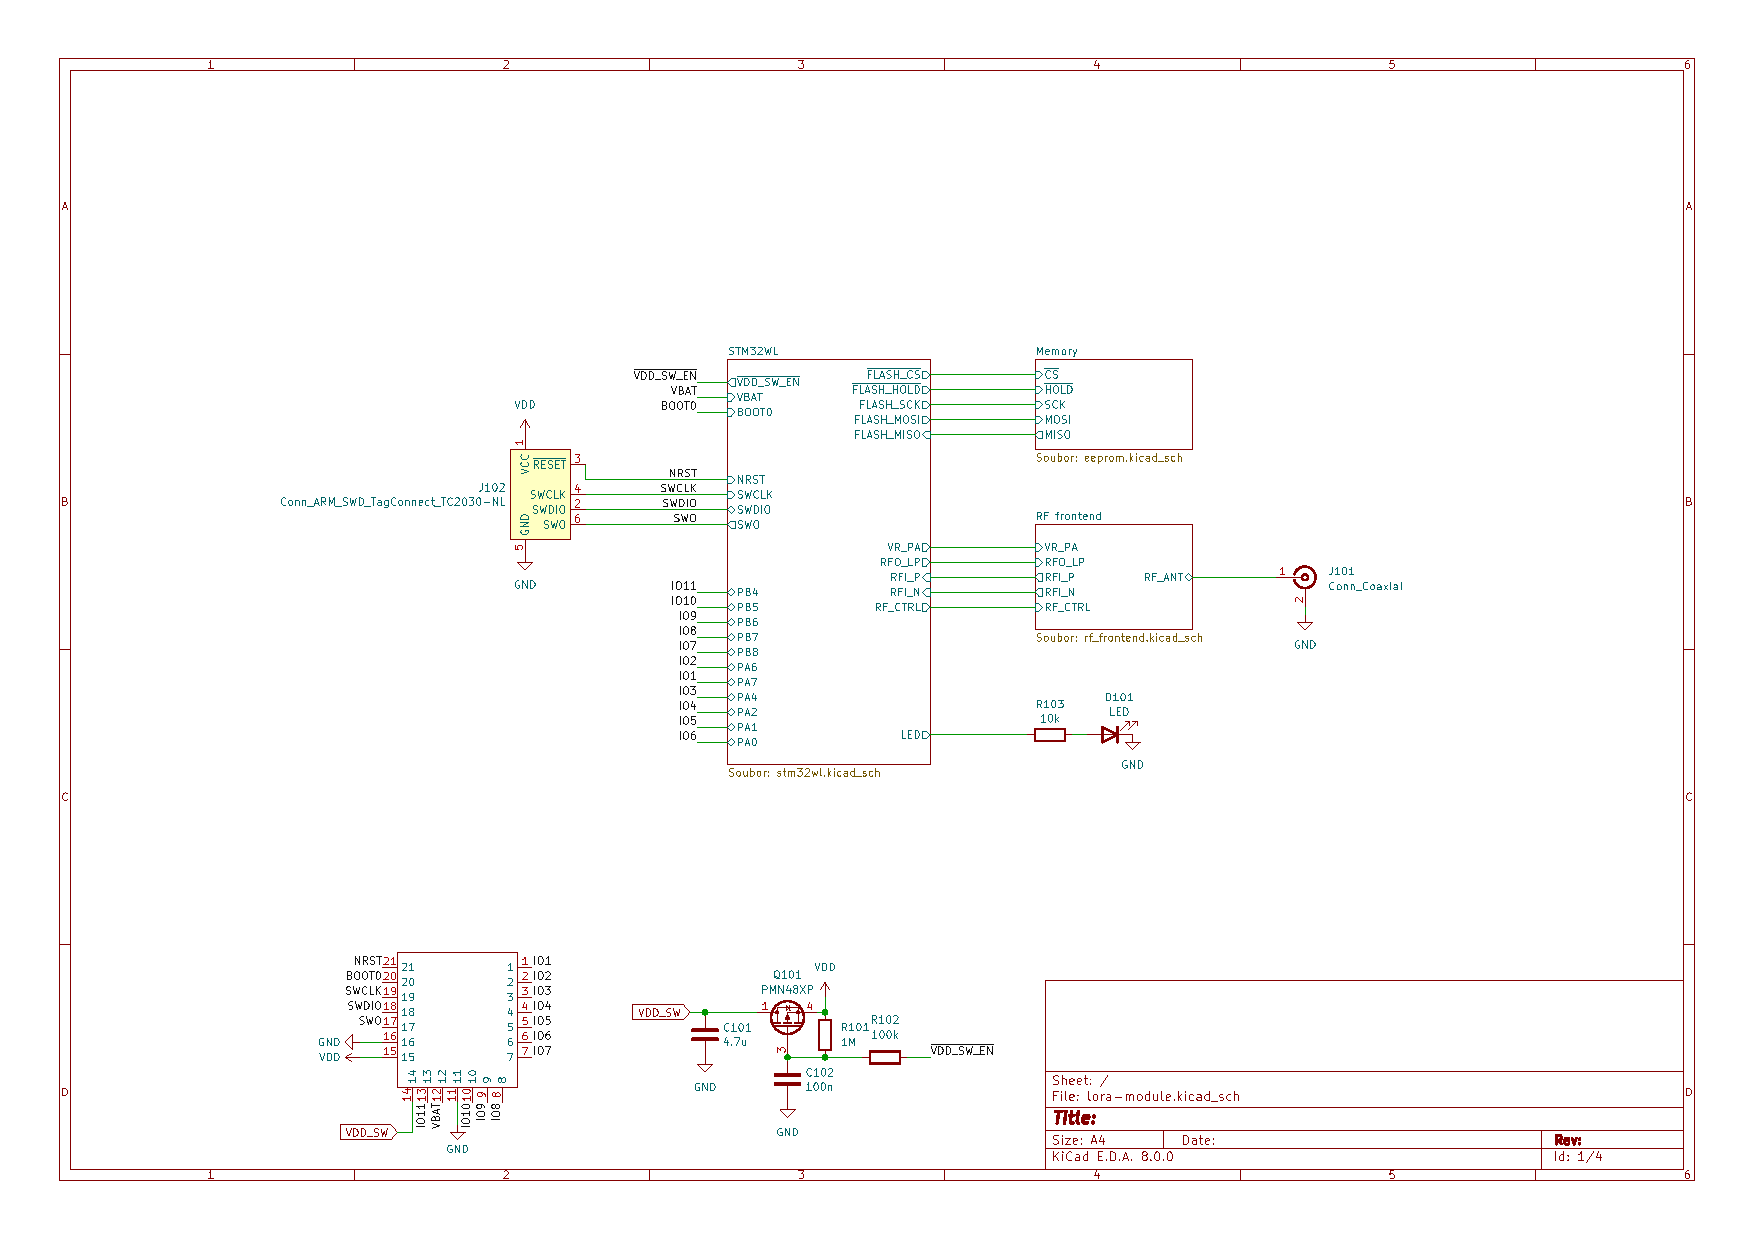
\includegraphics[page=1,angle=-90,width=\textwidth]{boards/v0.1/lora-module.pdf}
    \caption{\label{schematic:v0.1-1}Top level schematic sheet}
\end{figure}
\begin{figure}
    \includegraphics[page=2,angle=-90,width=\textwidth]{boards/v0.1/lora-module.pdf}
    \caption{\label{schematic:v0.1-2}STM32WLE5JC schematic sheet}
\end{figure}
\begin{figure}
    \includegraphics[page=3,angle=-90,width=\textwidth]{boards/v0.1/lora-module.pdf}
    \caption{\label{schematic:v0.1-3}RF frontend schematic sheet}
\end{figure}
\begin{figure}
    \includegraphics[page=4,angle=-90,width=\textwidth]{boards/v0.1/lora-module.pdf}
    \caption{\label{schematic:v0.1-4}Non-volatile memory schematic sheet}
\end{figure}

\begin{figure}
    \subfloat[Front layer]{\includesvg[width=.48\textwidth]{boards/v0.1/lora-module-F_Cu.svg}}\hfill
    \subfloat[Back layer]{\includesvg[width=.48\textwidth]{boards/v0.1/lora-module-B_Cu.svg}}\hfill
    \subfloat[Inner GND layer]{\includesvg[width=.48\textwidth]{boards/v0.1/lora-module-In1_Cu.svg}}\hfill
    \subfloat[Inner VCC layer]{\includesvg[width=.48\textwidth]{boards/v0.1/lora-module-In2_Cu.svg}}
    \caption{\label{board:v0.1}Module v0.1 PCB layer design}
\end{figure}

\begin{figure}
    \includesvg[width=\textwidth]{boards/v0.1/lora-module-F_Fab.svg}
    \caption{\label{board:v0.1-components}Module v0.1 component position reference}
\end{figure}
